
\documentclass[dvipdfmx]{standalone}
\usepackage[T1]{fontenc}
\usepackage{newtxtext, newtxmath}

\usepackage{tikz} % xcolor -> graphicx -> tikz
% \usetikzlibrary{fit}
% calc, positioning, quotes, topaths, scopes, spy
% matrix, graphs, graph.standard, trees, chains, automata, mindmap, er, calendar
% shapes.(geometric|symbols|arrows|multipart|callouts|misc)?
% arrows, patterns, fadings, shadings, shadows, backgrounds
% circuits.logic.US, circuits.ee.IEC, lindenmayersystems, folding, petri, svg.path
% decorations.(pathmorphing|pathreplacing|markings|footprints|shapes|text|fractals)?
% datavisualization, datavisualization.formats.functions
% intersections, plothandlers, plotmarks, through

\begin{document}
  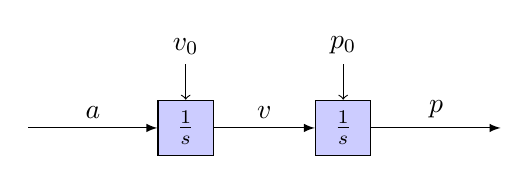
\begin{tikzpicture}[> = latex]
    \tikzset{
      int/.style={draw, fill=blue!20, minimum size=2em},
      init/.style={pin edge={to-,thin,black}},
    }
    \node [int, pin={[init]above:$v_0$}] (a) {$\frac{1}{s}$};
    \node (b) [left of=a, node distance=2cm, coordinate] {a};
    \node [int, pin={[init]above:$p_0$}] (c) [right of=a, node distance=2cm] {$\frac{1}{s}$};
    \node [coordinate] (end) [right of=c, node distance=2cm]{};
    \path[->] (b) edge node[above] {$a$} (a);
    \path[->] (a) edge node[above] {$v$} (c);
    \draw[->] (c) edge node[above] {$p$} (end) ;

  \end{tikzpicture}
\end{document}
